\documentclass[tikz, border=10pt]{standalone}
\usepackage{tikz}
\usetikzlibrary{positioning, arrows.meta, shapes, fit, calc}

\begin{document}
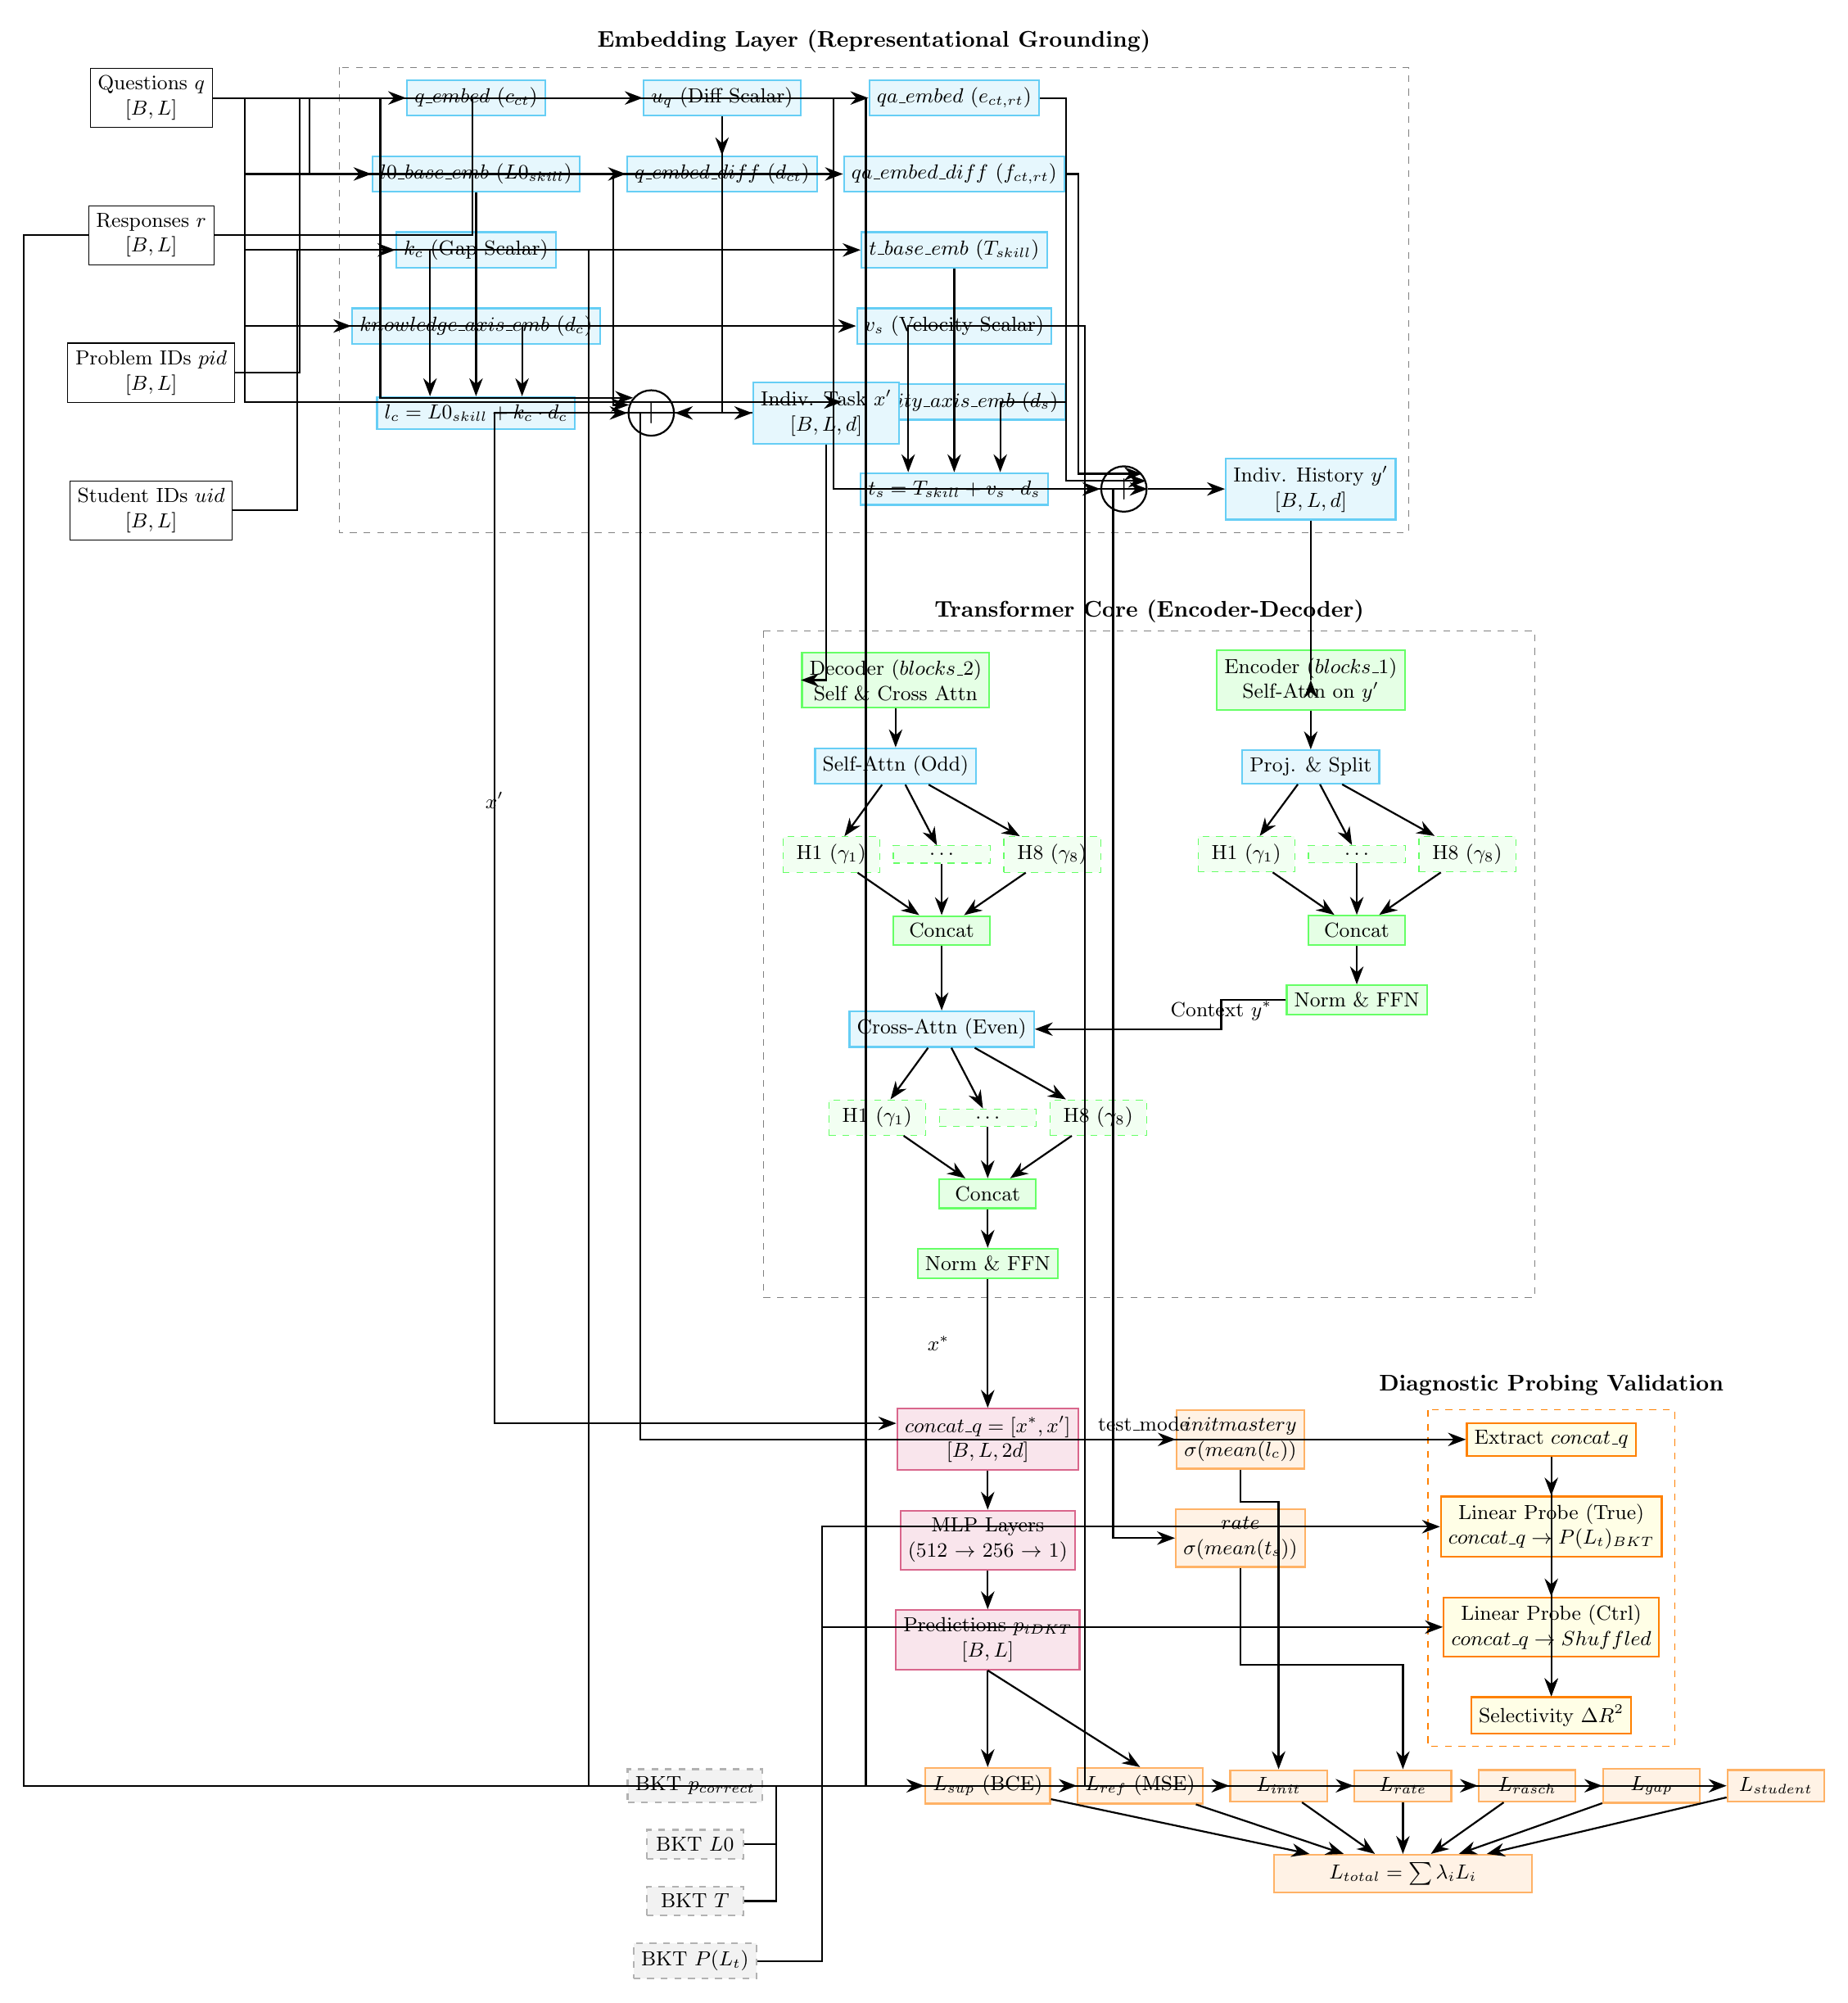
\begin{tikzpicture}[
    every node/.style={draw, rectangle, minimum width=1.5cm, align=center, font=\small},
    plain/.style={fill=white, draw=black},
    emb/.style={fill=cyan!10, draw=cyan!60, thick},
    attn/.style={fill=green!10, draw=green!60, thick},
    pred/.style={fill=purple!10, draw=purple!60, thick},
    loss/.style={fill=orange!10, draw=orange!60, thick},
    heads/.style={fill=green!5, draw=green!60, dashed},
    ref/.style={fill=gray!10, draw=gray!60, thick, dashed},
    plus/.style={fill=white, draw=black, thick, font=\Large, circle, inner sep=2pt, minimum width=0pt},
    probe/.style={fill=yellow!10, draw=orange, thick},
    arrow/.style={-{Stealth[scale=1.2]}, thick},
    label_node/.style={draw=none, fill=none, font=\bfseries}
    ]

    % ==========================================
    % 1. Input Layer
    % ==========================================
    \begin{scope}[local bounding box=input_box]
        \node[plain] (Input_q) {Questions $q$ \\ $[B, L]$};
        \node[plain, below=1.2cm of Input_q] (Input_r) {Responses $r$ \\ $[B, L]$};
        \node[plain, below=1.2cm of Input_r] (Input_pid) {Problem IDs $pid$ \\ $[B, L]$};
        \node[plain, below=1.2cm of Input_pid] (Input_uid) {Student IDs $uid$ \\ $[B, L]$};
    \end{scope}

    % ==========================================
    % 2. Embedding Layer (Grounding)
    % ==========================================
    \begin{scope}[local bounding box=emb_box]
        % Task Grounding Path (x')
        \node[emb, right=3cm of Input_q] (Base_Q) {$q\_embed$ ($c_{ct}$)};
        \node[emb, below=0.6cm of Base_Q] (L0_Base) {$l0\_base\_emb$ ($L0_{skill}$)};
        \node[emb, below=0.6cm of L0_Base] (Gap_Param) {$k_c$ (Gap Scalar)};
        \node[emb, below=0.6cm of Gap_Param] (K_Axis) {$knowledge\_axis\_emb$ ($d_c$)};
        \node[emb, below=0.8cm of K_Axis] (Formula_L0) {$l_c = L0_{skill} + k_c \cdot d_c$};

        % Shared Rasch Logic
        \node[emb, right=1.5cm of Base_Q] (Diff_Param) {$u_q$ (Diff Scalar)};
        \node[emb, below=0.6cm of Diff_Param] (Q_Diff) {$q\_embed\_diff$ ($d_{ct}$)};

        % History Grounding Path (y')
        \node[emb, right=5cm of Base_Q] (Base_QA) {$qa\_embed$ ($e_{ct,rt}$)};
        \node[emb, below=0.6cm of Base_QA] (QA_Diff) {$qa\_embed\_diff$ ($f_{ct,rt}$)};
        \node[emb, below=0.6cm of QA_Diff] (T_Base) {$t\_base\_emb$ ($T_{skill}$)};
        \node[emb, below=0.6cm of T_Base] (Vel_Param) {$v_s$ (Velocity Scalar)};
        \node[emb, below=0.6cm of Vel_Param] (V_Axis) {$velocity\_axis\_emb$ ($d_s$)};
        \node[emb, below=0.8cm of V_Axis] (Formula_T) {$t_s = T_{skill} + v_s \cdot d_s$};

        % Fusion Layer
        \node[plus, right=0.8cm of Formula_L0] (Sum_X) {+};
        \node[plus, right=0.8cm of Formula_T] (Sum_Y) {+};

        \node[emb, right=1.2cm of Sum_X] (Final_Q) {Indiv. Task $x'$ \\ $[B, L, d]$};
        \node[emb, right=1.2cm of Sum_Y] (Final_QA) {Indiv. History $y'$ \\ $[B, L, d]$};
    \end{scope}
    
    \node[label_node, above=0.3cm of emb_box] {Embedding Layer (Representational Grounding)};
    \draw[dashed, gray] ($(emb_box.north west)+(-0.2,0.2)$ ) rectangle ($(emb_box.south east)+(0.2,-0.2)$ );

    % ==========================================
    % 3. Transformer Core
    % ==========================================
    \begin{scope}[local bounding box=core_box]
        % Encoder
        \node[attn, below=2cm of Final_QA] (Enc_Desc) {Encoder ($blocks\_1$)\\Self-Attn on $y'$};
        \node[emb, below=0.6cm of Enc_Desc] (E_Split) {Proj. \& Split};
        \node[heads, below=0.8cm of E_Split, xshift=-1cm] (E_H1) {H1 ($\gamma_1$)};
        \node[heads, right=0.2cm of E_H1] (E_H2) {$\dots$};
        \node[heads, right=0.2cm of E_H2] (E_H8) {H8 ($\gamma_8$)};
        \node[attn, below=0.8cm of E_H2] (E_Concat) {Concat};
        \node[attn, below=0.6cm of E_Concat] (E_W) {Norm \& FFN};

        % Decoder
        \node[attn, left=3.5cm of Enc_Desc] (Dec_Desc) {Decoder ($blocks\_2$)\\Self \& Cross Attn};
        \node[emb, below=0.6cm of Dec_Desc] (KR1_Split) {Self-Attn (Odd)};
        \node[heads, below=0.8cm of KR1_Split, xshift=-1cm] (KR1_H1) {H1 ($\gamma_1$)};
        \node[heads, right=0.2cm of KR1_H1] (KR1_H2) {$\dots$};
        \node[heads, right=0.2cm of KR1_H2] (KR1_H8) {H8 ($\gamma_8$)};
        \node[attn, below=0.8cm of KR1_H2] (KR1_Concat) {Concat};

        \node[emb, below=1cm of KR1_Concat] (KR2_Split) {Cross-Attn (Even)};
        \node[heads, below=0.8cm of KR2_Split, xshift=-1cm] (KR2_H1) {H1 ($\gamma_1$)};
        \node[heads, right=0.2cm of KR2_H1] (KR2_H2) {$\dots$};
        \node[heads, right=0.2cm of KR2_H2] (KR2_H8) {H8 ($\gamma_8$)};
        \node[attn, below=0.8cm of KR2_H2] (KR2_Concat) {Concat};
        \node[attn, below=0.6cm of KR2_Concat] (KR2_FFN) {Norm \& FFN};
    \end{scope}

    \node[label_node, above=0.3cm of core_box] {Transformer Core (Encoder-Decoder)};
    \draw[dashed, gray] ($(core_box.north west)+(-0.3,0.3)$ ) rectangle ($(core_box.south east)+(0.3,-0.3)$ );

    % ==========================================
    % 4. Output Processing
    % ==========================================
    \begin{scope}[local bounding box=output_box]
        \node[pred, below=2cm of KR2_FFN] (Concat) {$concat\_q = [x^*, x']$ \\ $[B, L, 2d]$};
        \node[pred, below=0.6cm of Concat] (mlp_layers) {MLP Layers\\(512 $\to$ 256 $\to$ 1)};
        \node[pred, below=0.6cm of mlp_layers] (Pred) {Predictions $p_{iDKT}$ \\ $[B, L]$};

        \node[loss, right=1.5cm of Concat] (M_Init) {$initmastery$ \\ $\sigma(mean(l_c))$};
        \node[loss, below=0.6cm of M_Init] (M_Rate) {$rate$ \\ $\sigma(mean(t_s))$};
    \end{scope}

    % Diagnostic Probing
    \begin{scope}[local bounding box=probe_box, xshift=8cm]
        \node[probe, right=6cm of Concat] (Probe_Extract) {Extract $concat\_q$};
        \node[probe, below=0.6cm of Probe_Extract] (Probe_True) {Linear Probe (True)\\$concat\_q \to P(L_t)_{BKT}$};
        \node[probe, below=0.6cm of Probe_True] (Probe_Control) {Linear Probe (Ctrl)\\$concat\_q \to Shuffled$};
        \node[probe, below=0.6cm of Probe_Control] (Probe_Metric) {Selectivity $\Delta R^2$};
    \end{scope}
    
    \node[label_node, above=0.3cm of probe_box] {Diagnostic Probing Validation};
    \draw[dashed, orange] ($(probe_box.north west)+(-0.2,0.2)$ ) rectangle ($(probe_box.south east)+(0.2,-0.2)$ );

    % ==========================================
    % 5. Loss & Reference Data
    % ==========================================
    \begin{scope}[local bounding box=loss_box]
        \node[loss, below=1.5cm of Pred] (L_SUP) {$L_{sup}$ (BCE)};
        \node[loss, right=0.4cm of L_SUP] (L_REF) {$L_{ref}$ (MSE)};
        \node[loss, right=0.4cm of L_REF] (L_INIT) {$L_{init}$};
        \node[loss, right=0.4cm of L_INIT] (L_RATE) {$L_{rate}$};
        \node[loss, right=0.4cm of L_RATE] (L_RASCH) {$L_{rasch}$};
        \node[loss, right=0.4cm of L_RASCH] (L_GAP) {$L_{gap}$};
        \node[loss, right=0.4cm of L_GAP] (L_STUDENT) {$L_{student}$};
        \node[loss, below=0.8cm of L_RATE, minimum width=4cm] (L_TOTAL) {$L_{total} = \sum \lambda_i L_i$};
    \end{scope}

    \begin{scope}[local bounding box=ref_box]
        \node[ref, left=2.5cm of L_SUP] (BKT_P) {BKT $p_{correct}$};
        \node[ref, below=0.4cm of BKT_P] (BKT_L0) {BKT $L0$};
        \node[ref, below=0.4cm of BKT_L0] (BKT_T) {BKT $T$};
        \node[ref, below=0.4cm of BKT_T] (BKT_Mastery) {BKT $P(L_t)$};
    \end{scope}

    % ==========================================
    % WIRING (Arrows)
    % ==========================================
    
    % Input to Grounding
    \draw[arrow] (Input_q.east) -- ++(0.5,0) |- (Base_Q.west);
    \draw[arrow] (Input_q.east) -- ++(0.5,0) |- (L0_Base.west);
    \draw[arrow] (Input_q.east) -- ++(0.5,0) |- (T_Base.west);
    \draw[arrow] (Input_q.east) -- ++(0.5,0) |- (K_Axis.west);
    \draw[arrow] (Input_q.east) -- ++(0.5,0) |- (V_Axis.west);
    \draw[arrow] (Input_q.east) -- ++(1.5,0) |- (Q_Diff.west);
    
    \draw[arrow] (Input_pid.east) -- ++(1,0) |- (Diff_Param.west);
    \draw[arrow] (Input_uid.east) -- ++(1,0) |- (Gap_Param.west);
    \draw[arrow] (Input_uid.east) -- ++(1,0) |- (Vel_Param.west);
    
    \draw[arrow] (Input_r.east) -- ++(4,0) |- (Base_QA.west);
    \draw[arrow] (Input_r.east) -- ++(4,0) |- (QA_Diff.west);

    % Substantiation Formulas
    \draw[arrow] (L0_Base) -- (Formula_L0);
    \draw[arrow] (Gap_Param.east) -| (Formula_L0.160);
    \draw[arrow] (K_Axis.east) -| (Formula_L0.20);
    
    \draw[arrow] (T_Base) -- (Formula_T);
    \draw[arrow] (Vel_Param.east) -| (Formula_T.160);
    \draw[arrow] (V_Axis.east) -| (Formula_T.20);

    % Rasch Logic Connections
    \draw[arrow] (Diff_Param) -- (Q_Diff);

    % Fusion Wiring
    \draw[arrow] (Formula_L0) -- (Sum_X);
    \draw[arrow] (Q_Diff.west) -- ++(-0.2,0) |- (Sum_X.160);
    \draw[arrow] (Base_Q.west) -- ++(-0.4,0) |- (Sum_X.140);
    \draw[arrow] (Diff_Param.south) |- (Sum_X.east);
    
    \draw[arrow] (Formula_T) -- (Sum_Y);
    \draw[arrow] (Base_QA.east) -- ++(0.4,0) |- (Sum_Y.20);
    \draw[arrow] (QA_Diff.east) -- ++(0.2,0) |- (Sum_Y.40);
    \draw[arrow] (Diff_Param.east) -- ++(0.5,0) |- (Sum_Y.0);

    \draw[arrow] (Sum_X) -- (Final_Q);
    \draw[arrow] (Sum_Y) -- (Final_QA);

    % Transformer Core Wiring
    \draw[arrow] (Final_QA) |- (Enc_Desc);
    \draw[arrow] (Enc_Desc) -- (E_Split);
    \draw[arrow] (E_Split) -- (E_H1);
    \draw[arrow] (E_Split) -- (E_H2);
    \draw[arrow] (E_Split) -- (E_H8);
    \draw[arrow] (E_H1) -- (E_Concat);
    \draw[arrow] (E_H2) -- (E_Concat);
    \draw[arrow] (E_H8) -- (E_Concat);
    \draw[arrow] (E_Concat) -- (E_W);

    \draw[arrow] (Final_Q) |- (Dec_Desc);
    \draw[arrow] (Dec_Desc) -- (KR1_Split);
    \draw[arrow] (KR1_Split) -- (KR1_H1);
    \draw[arrow] (KR1_Split) -- (KR1_H2);
    \draw[arrow] (KR1_Split) -- (KR1_H8);
    \draw[arrow] (KR1_H1) -- (KR1_Concat);
    \draw[arrow] (KR1_H2) -- (KR1_Concat);
    \draw[arrow] (KR1_H8) -- (KR1_Concat);
    \draw[arrow] (KR1_Concat) -- (KR2_Split);
    
    \draw[arrow] (E_W.west) -- ++(-1,0) |- (KR2_Split.east) node[midway, above, sloped, draw=none, fill=none] {Context $y^*$};
    
    \draw[arrow] (KR2_Split) -- (KR2_H1);
    \draw[arrow] (KR2_Split) -- (KR2_H2);
    \draw[arrow] (KR2_Split) -- (KR2_H8);
    \draw[arrow] (KR2_H1) -- (KR2_Concat);
    \draw[arrow] (KR2_H2) -- (KR2_Concat);
    \draw[arrow] (KR2_H8) -- (KR2_Concat);
    \draw[arrow] (KR2_Concat) -- (KR2_FFN);

    % Output Wiring
    \draw[arrow] (KR2_FFN) -- (Concat) node[midway, left, draw=none, fill=none] {$x^*$};
    \draw[arrow] (Final_Q.west) -- ++(-4,0) |- (Concat.170) node[pos=0.2, above, draw=none, fill=none] {$x'$};
    \draw[arrow] (Concat) -- (mlp_layers);
    \draw[arrow] (mlp_layers) -- (Pred);
    
    \draw[arrow] (Formula_L0.east) -- ++(1,0) |- (M_Init.west);
    \draw[arrow] (Formula_T.east) -- ++(1,0) |- (M_Rate.west);

    % Probing Wiring
    \draw[arrow] (Concat.east) -- ++(1,0) |- (Probe_Extract.west) node[pos=0.5, above, draw=none, fill=none] {test\_mode};
    \draw[arrow] (Probe_Extract) -- (Probe_True);
    \draw[arrow] (Probe_Extract) -- (Probe_Control);
    \draw[arrow] (BKT_Mastery.east) -- ++(1,0) |- (Probe_True.west);
    \draw[arrow] (BKT_Mastery.east) -- ++(1,0) |- (Probe_Control.west);
    \draw[arrow] (Probe_True) -- (Probe_Metric);
    \draw[arrow] (Probe_Control) -- (Probe_Metric);

    % Loss Wiring
    \draw[arrow] (Pred.south) -- (L_SUP.north);
    \draw[arrow] (Input_r.west) -- ++(-1,0) |- (L_SUP.west);
    \draw[arrow] (Pred.south) -- (L_REF.north);
    \draw[arrow] (BKT_P.east) -- (L_REF.west);
    
    \draw[arrow] (M_Init.south) -- ++(0,-0.5) -| (L_INIT.north);
    \draw[arrow] (BKT_L0.east) -- ++(0.5,0) |- (L_INIT.west);
    
    \draw[arrow] (M_Rate.south) -- ++(0,-1.5) -| (L_RATE.north);
    \draw[arrow] (BKT_T.east) -- ++(0.5,0) |- (L_RATE.west);
    
    \draw[arrow] (Diff_Param.east) -- ++(1,0) |- (L_RASCH.west);
    \draw[arrow] (Gap_Param.east) -- ++(0.5,0) |- (L_GAP.west);
    \draw[arrow] (Vel_Param.east) -- ++(0.5,0) |- (L_STUDENT.west);
    
    \draw[arrow] (L_SUP) -- (L_TOTAL);
    \draw[arrow] (L_REF) -- (L_TOTAL);
    \draw[arrow] (L_INIT) -- (L_TOTAL);
    \draw[arrow] (L_RATE) -- (L_TOTAL);
    \draw[arrow] (L_RASCH) -- (L_TOTAL);
    \draw[arrow] (L_GAP) -- (L_TOTAL);
    \draw[arrow] (L_STUDENT) -- (L_TOTAL);

\end{tikzpicture}
\end{document}